\textbf{d)} Use van Kampen para calcular el grupo fundamental de la figura ocho.
\begin{proof}[\textbf{Solución}]
Sean $C_1$ y $C_2$ copias homeomorfas de $S^1$ con $C_1\cap C_2=\{q\}$. Tomemos $Y=C_1\cup C_2$ (figura ocho), $p\in C_1\setminus\{q\}$ y $r\in C_2\setminus\{q\}$.
\begin{center}
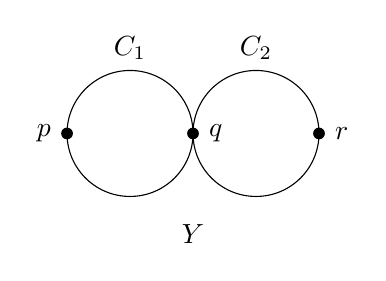
\begin{tikzpicture}[scale=0.8,dot/.style={circle,fill,inner sep=1.5pt}]
\draw (-1,0) circle (1);
\draw (1,0) circle (1);
\node[dot,label=left:$p$] at (-2,0) {};
\node[dot,label=right:$q$] at (0,0) {};
\node[dot,label=right:$r$] at (2,0) {};
\node at (-1,1.35) {$C_1$};
\node at (1,1.35) {$C_2$};
\node at (0,-1.6) {$Y$};
\end{tikzpicture}
\end{center}
Tomemos $U=Y\setminus\{p\}$ y $V=Y\setminus\{r\}$. Como $Y\setminus U=\{p\}\overset{\text{cer}}{\subseteq}Y$ y $Y\setminus V=\{r\}\overset{\text{cer}}{\subseteq}Y$ entonces $U\subseteqab Y$ y $V\subseteqab Y$. Además $Y=U\cup V$. Tenemos que $U$, $V$ y $U\cap V=Y\setminus\{p,r\}$ son conexos por caminos.
\begin{center}
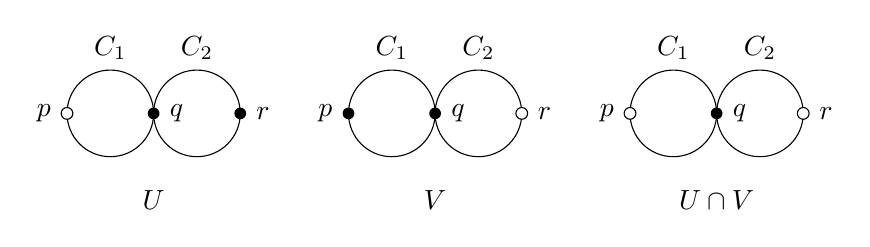
\begin{tikzpicture}[x=0.55cm,y=0.55cm,
dot/.style={circle,fill,inner sep=1.5pt},
hole/.style={circle,draw,fill=white,inner sep=1.5pt},
pics/eight/.style 2 args={code={
\draw (-1,0) circle (1);
\draw (1,0) circle (1);
\node[#1,label=left:$p$] at (-2,0) {};
\node[dot,label=right:$q$] at (0,0) {};
\node[#2,label=right:$r$] at (2,0) {};
\node at (-1,1.5) {$C_1$};
\node at (1,1.5) {$C_2$};
}}]
\pic at (-6.5,0) {eight={hole}{dot}};
\pic at (0,0) {eight={dot}{hole}};
\pic at (6.5,0) {eight={hole}{hole}};
\node at (-6.5,-2) {$U$};
\node at (0,-2) {$V$};
\node at (6.5,-2) {$U\cap V$};
\end{tikzpicture}
\end{center}
Como $U\cap V$ es homeomorfo al espacio estrellado
\begin{center}
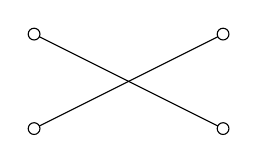
\begin{tikzpicture}[hole/.style={circle,draw,fill=white,inner sep=1.5pt}]
\draw (-1.2,0.6) -- (1.2,-0.6);
\draw (-1.2,-0.6) -- (1.2,0.6);
\node[hole] at (-1.2,0.6) {};
\node[hole] at (1.2,0.6) {};
\node[hole] at (-1.2,-0.6) {};
\node[hole] at (1.2,-0.6) {};
\end{tikzpicture}
\end{center}
entonces es simplemente conexo. Por tanto
\[
\pi_1(Y,q)\cong\pi_1(U,q)*\pi_1(V,q).
\]
Notemos que $U$ es homeomorfo al espacio $Z=S^1\cup(\{-1\}\times(-1,1))$ mediante una función que envía a $q$ en $q'=(-1,0)$.
\begin{center}
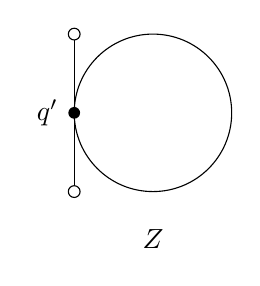
\begin{tikzpicture}[dot/.style={circle,fill,inner sep=1.5pt},hole/.style={circle,draw,fill=white,inner sep=1.5pt}]
\draw (0,0) circle (1);
\draw (-1,-1) -- (-1,1);
\node[hole] at (-1,1) {};
\node[hole] at (-1,-1) {};
\node[dot,label=left:$q'$] at (-1,0) {};
\node at (0,-1.6) {$Z$};
\end{tikzpicture}
\end{center}
Tenemos que $\{-1\}\times(-1,1)=(\{-1\}\times[-1,1])\cap Z\overset{\text{cer}}{\subseteq}Z$ y $S^1=S^1\cap Z\overset{\text{cer}}{\subseteq}Z$. Además, las funciones
\begin{align*}
H_1:(\{-1\}\times(-1,1))\times I&\to Z\\
((x,y),t)&\mapsto(x,(1-t)y)\\
H_2:S^1\times I&\to Z\\
((x,y),t)&\mapsto(x,y)
\end{align*}
son continuas, y $\operatorname{dom}(H_1)\cup\operatorname{dom}(H_2)=Z\times I$ con $\operatorname{dom}(H_1)\overset{\text{cer}}{\subseteq}Z\times I$ y $\operatorname{dom}(H_2)\overset{\text{cer}}{\subseteq}Z\times I$. Como también $H_1((-1,0),t)=(-1,0)=H_2((-1,0),t)$ para cualquier $t\in I$, y $\{(-1,0)\}\times I=\operatorname{dom}(H_1)\cap\operatorname{dom}(H_2)$, por el lema de pegado la función
\begin{align*}
H:Z\times I&\longrightarrow Z\\
((x,y),t)&\longmapsto
\begin{cases}
H_1((x,y),t) & \text{si } (x,y)\in\{-1\}\times(-1,1)\\
H_2((x,y),t) & \text{si } (x,y)\in S^1
\end{cases}
\end{align*}
es continua. Además
\begin{itemize}
\item Para cualquier $(x,y)\in Z$ se tiene
\begin{align*}
H((x,y),0)&=H_1((x,y),0)=(x,y) &&\text{si } (x,y)\in\{-1\}\times(-1,1),\\
H((x,y),0)&=H_2((x,y),0)=(x,y) &&\text{si } (x,y)\in S^1,\\
H((x,y),1)&=H_1((x,y),1)=(x,0)=(-1,0)\in S^1 &&\text{si } (x,y)\in\{-1\}\times(-1,1),\\
H((x,y),1)&=H_2((x,y),1)=(x,y)\in S^1 &&\text{si } (x,y)\in S^1.
\end{align*}
\item Para cualesquiera $(x,y)\in S^1$ y $t\in I$ se tiene $H((x,y),t)=H_2((x,y),t)=(x,y)$.
\end{itemize}
Por lo tanto $S^1$ es un retracto de deformación de $Z$, de modo que $\pi_1(U,q)\cong\pi_1(S^1,q)\cong(\mathbb{Z},+)$. Notemos que $U\cong V$ mediante una función que deja fijo a $q$, luego $\pi_1(V,q)\cong\pi_1(U,q)\cong(\mathbb{Z},+)$. De esta forma, $\pi_1(Y,q)\cong(\mathbb{Z},+)*(\mathbb{Z},+)$. Como $Y$ es conexo por caminos entonces para cualquier $y\in Y$ se tiene $\pi_1(Y,y)\cong\pi_1(Y,q)$ y por tanto $\pi_1(Y,y)\cong(\mathbb{Z},+)*(\mathbb{Z},+)$.
\end{proof}
